\documentclass[11pt, a4paper, UTF8]{ctexart}
\usepackage[body={14.64cm, 24.62cm}, centering, dvipdfm]{geometry}
\usepackage{fancyhdr}
\usepackage{listings}
\usepackage{color}
\usepackage{fontspec}
\usepackage{graphicx}
\usepackage{float}
\usepackage{extramarks}
\usepackage{amsmath}
\setmainfont{Times New Roman}
\setmonofont{Consolas}
\usepackage{tikz}
\usepackage{wallpaper}
\newcommand\BackgroundPicture{%
  \put(0,0){%
    \parbox[b][\paperheight]{\paperwidth}{%
      \vfill
      \centering%
        \begin{tikzpicture}[remember picture,overlay]
        \node [rotate=0,scale=1.1,text opacity=0.075] at (current page.center)
        { 
        	
\includegraphics{SJTU_BLUE.png}       %\copyright XXX Powered by~\LaTeX
        };
        \end{tikzpicture}%
%      \vfill
    }}}

\definecolor{mygreen}{rgb}{0,0.6,0}
\definecolor{mygray}{rgb}{0.5,0.5,0.5}
\definecolor{mymauve}{rgb}{0.58,0,0.82}

\newfontface\YaHeiMono{Microsoft YaHei Mono}
\newfontface\newSimSum{新宋体}

\lstset{ %
  backgroundcolor=\color{white},   % choose the background color; you must add \usepackage{color} or \usepackage{xcolor}
  basicstyle=\scriptsize \YaHeiMono,        % the size of the fonts that are used for the code
  breakatwhitespace=true,         % sets if automatic breaks should only happen at whitespace
  breaklines=true,                 % sets automatic line breaking
  captionpos=none,                    % sets the caption-position to bottom
  commentstyle=\color{mygreen} \newSimSum,
  morecomment=[l][\color{magenta}]{\#},    % comment style
  deletekeywords={...},            % if you want to delete keywords from the given language
  escapeinside={\%*}{*)},          % if you want to add LaTeX within your code
  extendedchars=true,              % lets you use non-ASCII characters; for 8-bits encodings only, does not work with UTF-8
  framexleftmargin=0.5em,
  frame=single,                    % adds a frame around the code
  keepspaces=true,                 % keeps spaces in text, useful for keeping indentation of code (possibly needs columns=flexible)
  keywordstyle=\color{blue},       % keyword style
  language=C++,                 % the language of the code
  otherkeywords={*,...},            % if you want to add more keywords to the set
  numbers=none,                    % where to put the line-numbers; possible values are (none, left, right)
  numbersep=1.5em,                   % how far the line-numbers are from the code
  numberstyle=\tiny\color{mygray}, % the style that is used for the line-numbers
  rulecolor=\color{black},         % if not set, the frame-color may be changed on line-breaks within not-black text (e.g. comments (green here))
  showspaces=false,                % show spaces everywhere adding particular underscores; it overrides 'showstringspaces'
  showstringspaces=false,          % underline spaces within strings only
  showtabs=false,                  % show tabs within strings adding particular underscores
  stepnumber=1,                    % the step between two line-numbers. If it's 1, each line will be numbered
  stringstyle=\color{red},     % string literal style
  tabsize=4,                       % sets default tabsize to 2 spaces
  title=\lstname,                   % show the filename of files included with \lstinputlisting; also try caption instead of title
  xleftmargin=2em,xrightmargin=2em  
}

\title{可持久化本地代码仓库——sit}
\author{柯嵩宇\quad 陈乐群 \\ 2014级ACM班 \\ 上海交通大学}

\fancyhead[L]{\textit{sit项目介绍}}
\fancyhead[C]{ACM班数据结构大作业(2015)}
\addtolength{\headheight}{12pt}

\begin{document}
\AddToShipoutPicture{\BackgroundPicture}

\pagestyle{fancy}
\maketitle
{\small \tableofcontents}
\newpage
\section{综述}
代码仓库在计算机科学的发展过程中扮演了一个非常重要的角色。一个优秀的代码仓库可以帮助程序员高效率地完成工作。这个学期的数据结构大作业,我们二人参考了git的设计编写了一个可持久化的本地代码仓库。

\section{项目简介}
\subsection{项目名称}
sit(a Simplified Git)
\subsection{支持的功能}
链式版本(即每个版本只有一个父版本)的保存与历史版本的检出以及对历史版本的修改。
\subsection{主要模块}
\begin{description}
	\item[Diff] 用于比较版本及文件间的差异。
	\item[FileSystem] 对boost::filesystem的封装,用于对文件的读写,复制及删除。
	\item[Index] 文件的索引相关的数据结构,用于保存某版本的文件的hash值。
	\item[Objects] 对版本的操作(保存文件,检出和重置版本)的数据结构的实现。
\end{description}
\subsection{主要命令}
\begin{description}
	\item[add] 把文件加入index。
	\item[checkout] 把指定的版本的文件(可以是单个文件,也可以是整个版本)复制到工作区。
	\item[commit] 将当前的index信息作为一个版本的全部文件信息并提交到仓库。
	\item[diff] 比较特定版本(全版本或特定文件)之间的差异。
	\item[init] 在当前的工作目录初始化一个版本仓库。
	\item[log] 输出已保存的版本的版本信息。
	\item[status] 输出当前工作区的文件信息。
	\item[reset] 将index或index中一个特定文件的信息重置为某个特定的版本。
	\item[rm] 将文件从index中移除。
\end{description}

\section{模块介绍}

\subsection{Color}
\subsubsection{简介}
高亮输出信息,增强可读性。
\subsubsection{实现方法}
\begin{description}
	\item[Windows] 通过Win32 API实现,颜色数量较少,实际效果较差。
	\item[Unix及其他POSIX标准系统] 通过ANSI颜色序列实现,色彩丰富,实际效果较好。
\end{description}

\subsection{Config}
\subsubsection{简介}
sit的配置模块,用来读取和修改作者信息(作者名字及Email地址)。

\subsection{Core}
\subsubsection{简介}
sit的核心模块,sit的所有命令都调用Core中相关函数实现。

\subsection{Diff}
\subsubsection{简介}
用于比较两个文件之间或两个版本之间的差异。
\subsubsection{实现方法}
\begin{description}
	\item[版本之间] 先对两个版本的index进行diff,等到两个版本的文件列表的额差异信息(Add, Rm, Modify, Same),然后对差异信息为Modify的文件调用针对文件的比较算法。
	\item[文件之间] 对两个文件逐行Hash,对得到的Hash值列表执行LCS算法(时间复杂度$O((n+m)*d)$,其中$n$, $m$为两个列表的长度,$d$为输入数据的差异个数)。
\end{description}

\subsection{Hash}
\subsubsection{简介}
Hash在本项目中扮演了非常重要的角色,包括版本的管理和Diff算法的实现。
\subsubsection{Hash在项目中的使用}
使用SHA1算法的Hash值作为文件名来保存文件。虽然效率上会受到一定的影响,但为了保证跨平台的兼容性,SHA1算法直接使用了boost库中的实现而不是git中使用了大量内嵌汇编的SHA1算法。

在针对文件的比较算法中,先使用了MurmurHash3的Hash算法,并且针对32bit和64bit的系统做出了针对性优化。

\subsection{FileSystem}
\subsubsection{简介}
由于Windows和Linux对文件操作的API各不相同,因此使用boost库中的filesystem进行文件操作。同时为了方便代码的编写和实现一些必要的操作,对boost::filesystem进行了再封装。
\subsubsection{主要函数}
\begin{description}
	\item[CompressCopy] 对源文件进行压缩后进行复制,主要用于add命令的实现。
	\item[CompressWrite] 将一个字符串压缩后写入文件,主要用于版本信息的压缩与写入。
	\item[DecompressCopy] 对源文件进行解压后进行复制,主要用于需要从版本库中复制文件的命令的实现。
	\item[DecompressRead] 对一个被压缩的文件使用,返回文件原来的信息,主要用于对版本信息的解压与读取。
	\item[GetRelativePath] 得到路径A相对于路径B的相对路径,用于保证在仓库的子目录中调用sit是可以得到正确的执行结果。
	\item[ListRecursive] 返回包含某一个目录下的所有文件的vector,主要用于实现需要文件夹递归的命令(add, checkout, etc)
\end{description}

\subsection{Index}
\subsubsection{简介}
程序运行时用于处理版本的文件列表信息的数据结构,其本质是对std::unordered\_map的再封装。
\subsubsection{实现细节}
考虑到在程序运行过程中需要处理三种类型的文件列表:
\begin{enumerate}
	\item 保存在".sit/index"中的已暂存的文件信息。
	\item 保存在".sit/objects"中以树形结构储存的文件信息。
	\item 当前工作目录下所有文件的文件信息。
\end{enumerate}
其中所有的文件列表都使用<路径,SHA1值>的键值对保存。

在项目中编写了基类IndexBase,以及其针对文件中的index信息的派生类CommitIndex、针对".sit/index"中的文件信息的派生类Index、针对当前工作目录的所有文件的派生类WorkingIndex。

文件列表的读取和写入通过FileSystem和Objects模块来实现。

\subsection{Objects}
\subsubsection{简介}
作为文件与Index之间的中间数据结构,在Index与Commit文件的转换中具有重要的作用。tree类型的object以树形结构保存了index中的文件列表,清晰地记录了文件和路径的关系。
\subsubsection{实现细节}
包含三种类型的Objects:
\begin{description}
	\item[commit] 该类型的object表示该文件记录的是一个版本信息,包含文件的信息和该commit的信息(作者,时间,以及COMMIT\_MSG)。
	\item[tree] 表示这个文件记录了一个文件列表,该object的内容是同一个文件夹下所有文件的信息,每行一个object,分别代表文件权限,该object的类型,SHA1值,以及object的名字(如果是blob类型则该文件的文件名,如果是tree类型,则表示该文件夹的名字)。
	\item[blob] 一个基本的object类型,表示它是路径树上的叶子节点,是原文件的一个副本。
\end{description}
保存Object的结构体:
\begin{lstlisting}
struct TreeItem {
	int mode;                         // Linux文件权限,如10644
	ObjectType type;                  // 这个Object的类型:tree or blob
	std::string id;                   // 文件的SHA1值,等价于文件的路径
	boost::filesystem::path filename; // 文件路径
};
\end{lstlisting}
保存Commit信息的结构体
\begin{lstlisting}
struct Commit {
	std::string tree;      // 以REPO_ROOT为根的目录树的SHA1 Hash值
	std::string parent;    // 该提交的父版本
	std::string author;    // 作者的名字,Email地址,时间戳,时区
	std::string committer; // 提交者的名字,Email地址,时间戳,时区
	std::string message;   // Commit Messages
};
\end{lstlisting}

\subsection{Refs}
\subsubsection{简介}
用于处理与版本指针相关的引用信息,如,当前工作区的版本(HEAD指针),当前分支的版本指针(指向当前分支的最后一个版本,由于sit目前不支持分支功能,故只有一个默认生成的master分支)。编写该模块的目的主要是为了减少以后需要增加分支功能的时候的工作量。

\subsection{Status}
\subsubsection{简介}
用于处理工作区和index以及版本库之间的关系,输出当前工作区的状态。
\subsubsection{实现细节}
使用Index模块中的WorkingIndex类生成包含当前工作区的所有文件信息的index,会与保存在``.sit/index''中的index以及HEAD指针所指向的commit比较,生成文件的状态(新增,修改,删除及这些改动是否被``.sit/index''所记录)。如果三者完全相同那么认为工作区是clean的。同时,工作区是clean的是checkout命令的对象为commit时能正确执行的前提。

\subsection{Util}
\subsubsection{简介}
重要的一个模块,作为整个工程的工具模块,包含了对boost库中SHA1算法的封装,以及根据当前的objects目录提供的SHA1值的补全功能,增强了sit的易用性。

该模块中定义了sit的异常类SitException,处理由于用户的非法操作造成的错误并给出说明。


\section{命令介绍}
sit使用了boost中的program\_options模块来格式化处理命令行参数。除了非默认参数外,其余参数在使用时均需要满足下列格式之一:
\begin{lstlisting}[language=sh]
--<option_name>=<option_value>
-<option_abbr>=<option_value>
\end{lstlisting}

其中等号可以用空格代替。默认参数可以省略掉等号前面的部分。

下文提到的{\YaHeiMono <commit-id>}都代表此处接受某个commit的SHA1值的足够长的前缀或版本指针的名字(如HEAD,index,work,master)。
\subsection{add}
\subsubsection* {Introduction}
把文件内容加入到index
\subsubsection*{Usage}
\begin{lstlisting}[language=sh]
sit add <path_1> [<path_2> ...]
\end{lstlisting}
\subsubsection*{Options}
\begin{description}
	\item[\YaHeiMono <path>(默认参数)] 要加入index的文件(或文件夹,如果是文件夹将递归加入该文件夹下所有的子文件(夹))
\end{description}

\subsection{checkout}
\subsubsection*{Introduction}
将代码库/index中的文件解压并复制到当前的工作区中。
\subsubsection*{Usage}
checkout命令有两种基本形式:
\begin{lstlisting}[language=sh]
sit chekcout [--commit=<commit-id>]
\end{lstlisting}
\begin{lstlisting}[language=sh]
sit checkout [--commit=<commit-id>] --path=<path_1> [--path=<path_2> ...]
\end{lstlisting}
\subsubsection*{Options}
\begin{description}
	\item[\YaHeiMono commit] 指定复制到工作区的文件来源,接受的值为任意一个commit的ID的前缀(可以自动补全)或者是版本指针(目前支持的有HEAD,index,master),默认值为index。
	\item[\YaHeiMono path(默认参数)] 指定需要复制到工作区的文件(夹),如果没有指定任何一个文件,那么checkout将复制该commit的所有文件到工作区,并且将HEAD指针指向checkout的commit(如果commit参数为index则不改变HEAD指针)。
\end{description}

\subsection{config}
\subsubsection*{Introduction}
修改该仓库的配置,目前支持的仓库配置有用户名和用户的Email地址(user.name和user.email)。
\subsubsection*{Usage}
\begin{lstlisting}[language=sh]
sit config <key> <value>
\end{lstlisting}
\subsubsection*{Options}
\begin{description}
	\item[\YaHeiMono <key>] 修改配置的字段名
	\item[\YaHeiMono <value>] 新的配置值
\end{description}

\subsection{commit}
\subsubsection*{Introduction}
将当前``.sit/index''文件中记录的文件信息写入仓库。
\subsubsection*{Usage}
\begin{lstlisting}[language=sh]
sit commit  [--amend] [--all | -a] [--message | -m COMMIT_MSG]
\end{lstlisting}
\subsubsection*{Options}
\begin{description}
	\item[\YaHeiMono all,a] 等价于在执行commit操作之前先执行一次`add <REPO\_ROOT>',其中REPO\_ROOT表示仓库的绝对路径。
	\item[\YaHeiMono amend] 表示新的commit将取代原来的HEAD所指向的commit在版本链中的位置。\\\textbf{注意:如果没有amend参数,那么commit只有当HEAD指针与master指针相等的时候才会执行(为了保证版本链的唯一)。}
	\item[\YaHeiMono message,m] 以参数的形式提供用于描述该commit改动的信息。
\end{description}

\subsection{diff}
\subsubsection*{Introduction}
比较两个commit的文件信息(或两个不同版本的同一文件(夹))的差异。
\subsubsection*{Usage}
\begin{lstlisting}[language=sh]
sit diff [--base-id=<commit-id>] [--target-id=<commit-id>] [--path=<path> ...]
\end{lstlisting}
\subsubsection*{Options}
\begin{description}
	\item[\YaHeiMono base-id] 作为基准的commit的ID,默认值为index。
	\item[\YaHeiMono target-id] 比较差异的commit的ID,默认值为work(即当前的工作区)。
	\item[\YaHeiMono path(默认参数)] 用于指定需要比较的文件(夹),如果没有指定任何一个文件,那么将比较两个版本的index以及每一个有修改的文件。
\end{description}

\subsection{gc}
\subsubsection*{Introduction}
删除那些``不再需要''的objects,释放它们占用的硬盘空间。
\subsubsection*{Usage}
\begin{lstlisting}[language=sh]
sit gc
\end{lstlisting}

\subsection{init}
\subsubsection*{Introduction}
在当前的工作目录下建立一个sit的版本仓库,如果已经存在了一个sit的版本仓库,那么将把这个版本仓库删除后再创建
(即初始化)。
\subsubsection*{Usage}
\begin{lstlisting}[language=sh]
sit init
\end{lstlisting}

\subsection{log}
\subsubsection*{Introduction}
以当前HEAD指针指向的commit为最后的commit,输出该commit以及它的所有父版本的信息(作者,提交时间,提交信息)。
\subsubsection*{Usage}
\begin{lstlisting}[language=sh]
sit log
\end{lstlisting}

\subsection{status}
\subsubsection*{Introduction}
将当前的工作区的index和HEAD指针所指向的commit的index进行比较,分别输出新增的文件、被修改的文件、被删除的文件的列表。
\subsubsection*{Usage}
\begin{lstlisting}[language=sh]
sit status
\end{lstlisting}

\subsection{reset}
\subsubsection*{Introduction}
将仓库中某个commit中保存的文件信息恢复到当前的index中。
\subsubsection*{Usage}
reset命令有两种形式:
\begin{lstlisting}[language=sh]
sit reset [--hard] [--commit=<commit-id>]
\end{lstlisting}
\begin{lstlisting}[language=sh]
sit reset  [--commit=<commit-id>] --path=<path_1> [--path=<path_2> ...]
\end{lstlisting}

第一种形式会将当前分支的版本指针移动到指定的commit上。(移动版本链的链表尾,操作后尾后的commit还会存在仓库中,此时执行gc命令将把这些commit相关的且没有被其他文件引用的objects清理掉。)

第二种形式必须指定最少要恢复的文件,否则sit会将其解释为第一种形式。
\subsubsection*{Options}
\begin{description}
	\item[\YaHeiMono hard] 如果给出``--hard''参数,那么reset命令在恢复index中的文件信息的同时,会从仓库中复制相应的文件到工作区。如果没有则reset命令只会对index进行修改。
	\item[\YaHeiMono commit] 用于指定要恢复到index的文件信息来自于哪一个commit,默认值为HEAD。
	\item[\YaHeiMono path(默认参数)] 用于指定恢复哪些文件的信息。\textbf{注意:path参数和hard参数不能同时存在。如果必要的话,可以先后执行reset和checkout两个命令来满足要求。}
\end{description}

\subsection{rm}
\subsubsection*{Introduction}
把文件(夹)的记录从index中移除,不会修改工作区的文件(夹)。
\subsubsection*{Usage}
\begin{lstlisting}[language=sh]
sit rm --path=<path_1> [--path=<path_2> ...]
\end{lstlisting}
\subsubsection*{Options}
\begin{description}
	\item[\YaHeiMono path(默认参数)] 表示要从index中移除的文件(夹)。
\end{description}

\section{设计上的考量}

\subsection{树形结构 vs列表列表}

在设计 Commit 的文件记录的时候,我们最初的想法是直接使用和
\texttt{index} 一样的列表方式,即 \texttt{(sha1,\ path)} 二元组:

\begin{lstlisting}[language=Clean,numbers=none]
87bbffd3a1c068111def6f38cf4e195aa08e9a37 utils/redis.conf.tpl
af10d3a3c39b16d476945a2767f09d963c939f87 utils/redis-sha1.rb
ee1a1142186d2f26d487dbb9297a4197926036b2 utils/install_server.sh
164a227ff04074c4fbd86bcd6881641c739a41b8 utils/help.h
237374c7b84f640b88742222eb161f2f2be566d3 utils/generate-command-help.rb
6ddbed31efd3d6c5c2148dd77cade28aa3542d75 utils/build-static-symbols.tcl
dcec114564d10da5bfc0e441c1cc13e6c3662ad6 tests/unit/type/zset.tcl
11ee092a91aa9dc28095d6a4a7012920c93b79b4 tests/unit/type/set.tcl
4d4a1185a19bdcb88a96bf5e5819032ebf4a0e2a tests/unit/type/list-common.tcl
ac2e98b25e3e84c4371ae12f2821713cac92e7dc tests/unit/type/list-3.tcl
\end{lstlisting}

然而,在参考了 git
的实现之后,我们选择了使用树形结构来实现我们的文件记录。我们引入
\texttt{tree} 和 \texttt{blob} 两个概念。 \texttt{tree}
表示的就是文件系统中的一个目录,而 \texttt{blob}
表示的就是一个目录中的文件。这样,我们的文件列表即变为类似这样的树形结构,即
\texttt{(type,\ object\ id,\ filename)} 的多元组:

\begin{lstlisting}[language=Clean,numbers=none]
tree e36c8aebd0c8d837f11af835ddf3c73d912abc2b src
tree c266ec6cfd9b89b337feb285c3dd3a1d45a6f04e tests
tree 9c9493aadc3d1faae7f0108d0465ccda9b3a0e6f utils
blob f8beb85f2fd472896df6cbee3c88f37c4f91df75 zip.c
blob f6f0ff0af6590f7ed077f889da5ea3748489994f ziplist.c
blob 88af6ae3e023bc924afee7852b359f69155aca74 ziplist.h
blob fa4b2ebfc54608bbf5f4c9642018879f317b4a97 zipmap.c
blob 2c969f4a1e7784a545c3e733299a7b08308c8010 zipmap.h
blob 1da2e22f30df5e329da57e41ced427603c8d8ebc zmalloc.c
blob 935bbb5627be626dbbdba0f86ca3f9f362ec9ea7 zmalloc.h
\end{lstlisting}

可以做如下估计:若采用列表方式,假设项目中有 65536
个文件,又假设平均路径长度为 22 个字符,那么加上 SHA1
值及换行符之后,一行需要 64 个字符,也就是说,单次 commit
的文件列表需要占用
\texttt{65536~*~64~Bytes~=~4~MBytes}。将以上假设应用于 Linux
内核约 500000 次提交,则光是维护文件列表就需要占用 \texttt{2~GBytes}
空间,这是一个相当大的浪费。

而采用树形结构来存储的话,每次提交只需要重建修改文件所在路径上所有父目录的
\texttt{tree}
对象。考虑到大型项目大致都有较为细分的目录结构,而且单次提交中修改的文件数量十分的少,因此在大型项目中的单次
commit 的文件列表占用空间就大大减小了。

\subsection{处理树形结构与列表结构}

虽然树形结构能节约很多的磁盘空间,然而在程序的处理过程中却并不容易,因此我们的做法是:在处理树形结构时先转换成内存中的列表结构,(如果有需要)再将列表结构转成树形结构写入磁盘。这么做虽然看起来比较浪费时间,但实际上每次运行
sit
时,这种转换的次数非常少。另外转换成列表后,程序的处理将变得更加简单和统一。

在 sit 执行各种任务时,会遇上以下几种不同的文件列表:

\begin{itemize}
\item
  树形结构
\item
  repo 目录的文件系统
\item
  commit 的文件列表
\item
  列表结构
\item
  stage 区的 index
\end{itemize}

sit 的各种任务比如 \texttt{diff}, \texttt{status}, \texttt{checkout},
\texttt{reset}
等,需要同时处理以上多种列表。为了方便实现和减少重复代码,我们使用了 C++
继承特性。

我们首先建立了基类 \texttt{IndexBase}
维护文件列表,支持对文件列表的查增删改。然后针对以上三种不同的文件列表,我们派生出了
\texttt{WorkingIndex}, \texttt{CommitIndex} 和 \texttt{Index}
这三个类,各自使用不同的方法读取列表及将列表写入文件。

这样一来,在 \texttt{diff}
等任务在处理时,无需关心当前处理的是哪一种列表,只需要向函数中传入
\texttt{IndexBase} 类型的变量即可,大大减少了重复代码以及繁冗的判断。

\subsection{diff 算法}

对两个文件执行 diff 操作,我们的实现方法是先将文件按行执行
hash,这样就得到了两个序列。于是就可以将两个文件执行 diff
操作转换为求两个序列的最长公共子序列 (LCS)。

在按行 hash 时,我们最先尝试使用 \texttt{std::hash},该函数能将
\texttt{std::string} hash 成为一个 \texttt{size\_t}
值,并且具有非常高的效率。然而我们随后发现,假设某个文件有 50000
行文字,那么在一台32位的机器上对这 50000 个字符串进行
hash,由生日攻击的方法可以算出冲突概率(假设hash结果均匀分布):

\[
100\%-\prod _{i=1}^{50000} \left(1-\frac{i-1}{2^{32}}\right) = 25.3 \%
\]

这是一个很糟糕的结果。而如果 hash 值提升到64位以上的话,在 50000
个字符串中冲突的概率几乎为0.

在得知 \texttt{std::hash} 使用了 \texttt{MurmurHash2}
算法后,最终我们选定了128位版本的 \texttt{MurmurHash3} 算法,这比32位的
\texttt{MurmurHash2} 算法拥有更高的效率和更低的冲突率。

在解决了 hash 问题后,重点就放在了解决 LCS 问题了。LCS
朴素的动态规划方法需要$O(N*M)$ 的时间及空间复杂度,其中
$N,\ M$
分别为两个字符串的长度。这并不是一个优秀的算法,时间复杂度和空间复杂度均不可接受。

经了解,\texttt{GNU\ diff} 和 \texttt{libxdiff} 这两个常用的 diff
工具所使用的 diff 方法都是基于 Eugene Myers 的论文 \emph{An O(ND)
Difference Algorithm and its Variations}。该算法期望时间复杂度为
$O(N+M+D^2)$ ,最坏时间复杂度为 $O((N+M)D)$
(可进一步优化至理论复杂度 $O((N+M)log(N+M)\ +\ D^2)$,其中
$D$ 为两个序列的差异大小),并且具有线性的空间复杂度。

我们实现了这个算法。因为在sit的应用场景中,同一个文件的两个版本差异并不会很大,因此这个
$O((N+M)D)$ 的算法获得了非常好的效果。

而 diff 算法还有许多进一步的优化空间,如:

\begin{itemize}
\item
  在差异过大的时候可以使用近似算法以保证在极短的时间内完成比较
\item
  LCS答案并不唯一,选择较优的方案输出
\end{itemize}

这两者在常见的 diff
程序中均有做出相应的优化,鉴于这些优化较为复杂,而且本次项目的重点并不在此,所以我们略过了这些优化。

\subsection{彩色输出}

Windows 下和 Unix 及 Linux 下的控制台彩色输出有所不同。在 Unix 和 Linux
中,可以直接向终端输出 ANSI 彩色序列来改变色彩,而在 Windows 中必须调用
Windows API 来实现。为了方便不同平台的彩色输出,我们重载了
\texttt{ostream} 的 \texttt{\textless{}\textless{}}
操作符,使得彩色输出变得异常的简便,如:

\begin{lstlisting}
cout << Color::RED << "Red" << Color::RESET << endl;
\end{lstlisting}


\section{压力测试}
从github上获取redis 2.4的版本仓库用于测试git与sit的时空效率。
\subsection{测试方法}
在redis中以master分支为基准,找出一条版本链,如果这个版本是merge得到的,那么就选择它的第一个父版本。然后将版本链上的每一个版本checkout,然后执行add和commit命令,同时监控其CPU时间的消耗。
\subsection{空间占用}
把所有的文件都add和commit到仓库中后分别查看``.sit''和``.git''文件夹的大小。
\begin{center}
\begin{tabular}{|l|r|r|}
\hline
                         & 仓库大小 & 相对大小\\
\hline
.git                     & 94324 kB           &   100\% \\
\hline
.sit(with compression)   & 82180 kB           &  87.1\% \\
\hline
.sit(without compression)& 264004 kB          & 279.9\% \\
\hline
\end{tabular}
\end{center}
\subsection{时间使用}
比较了sit(有无压缩功能)与git的时间效率(结果见后图)。
\begin{figure}[H]
	\centering
	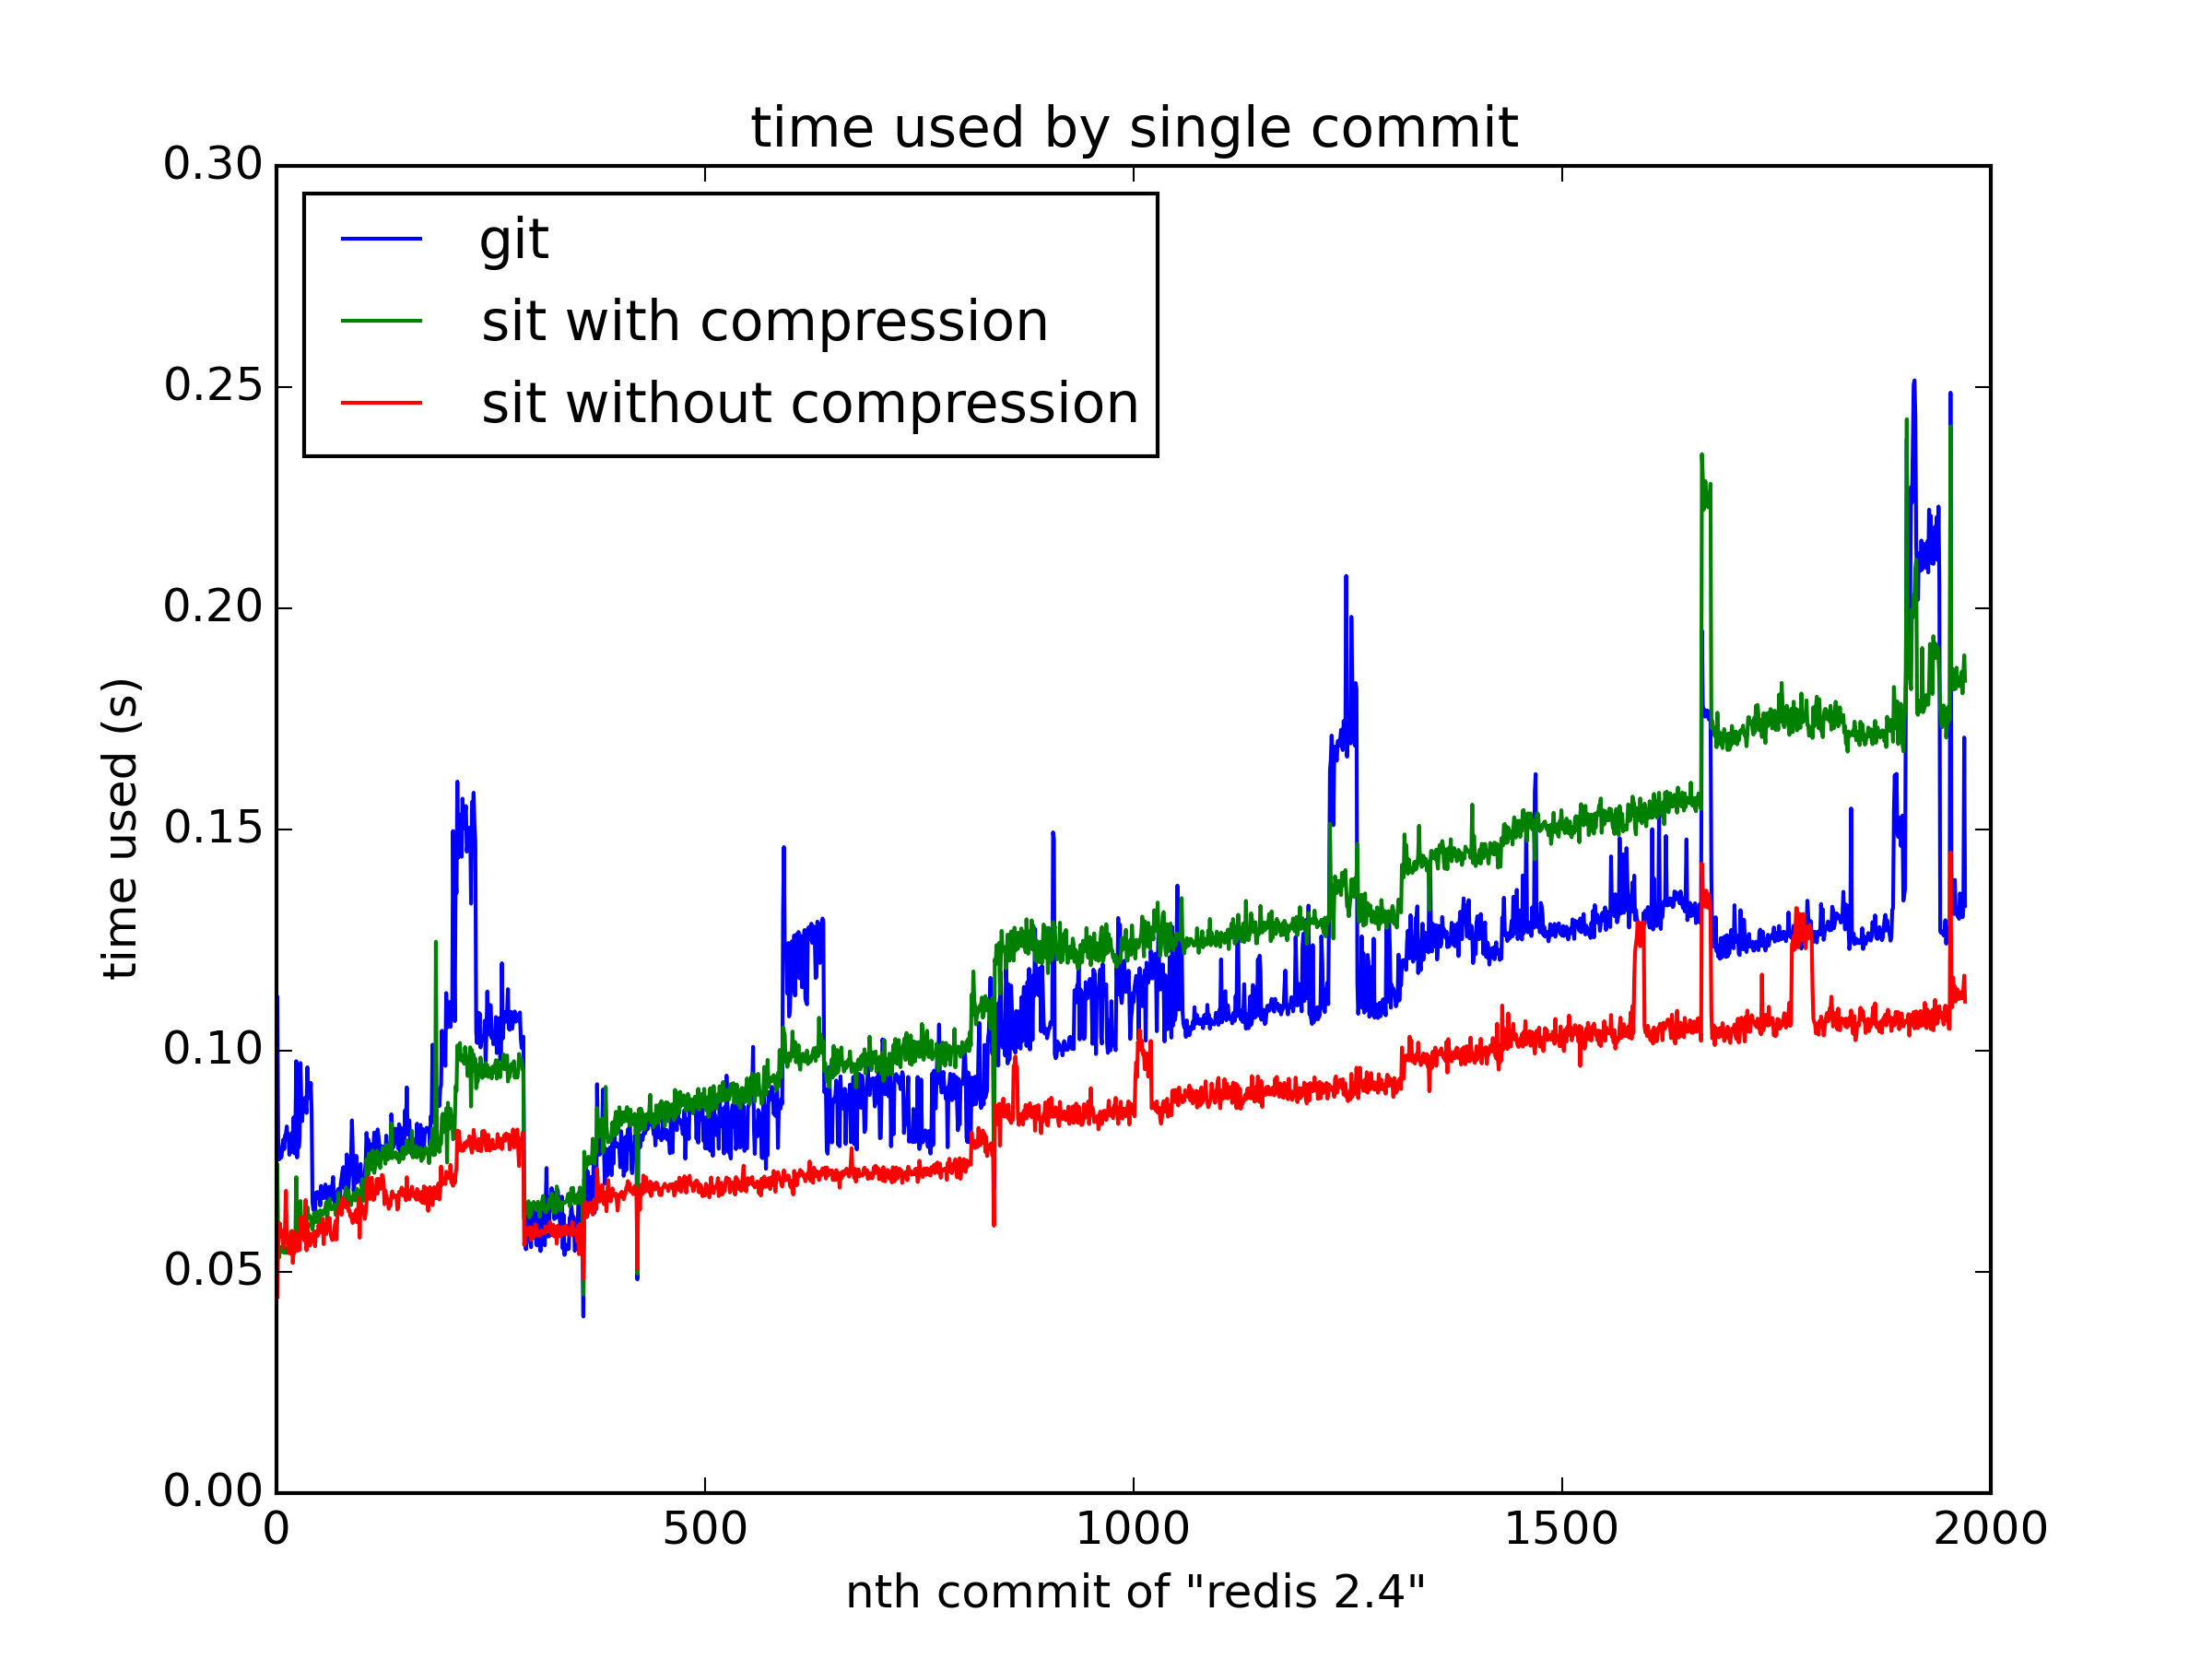
\includegraphics[scale=0.7]{figure_1.png}
	\caption{单次commit操作所需要的时间}
\end{figure}
\begin{figure}[H]
	\centering
	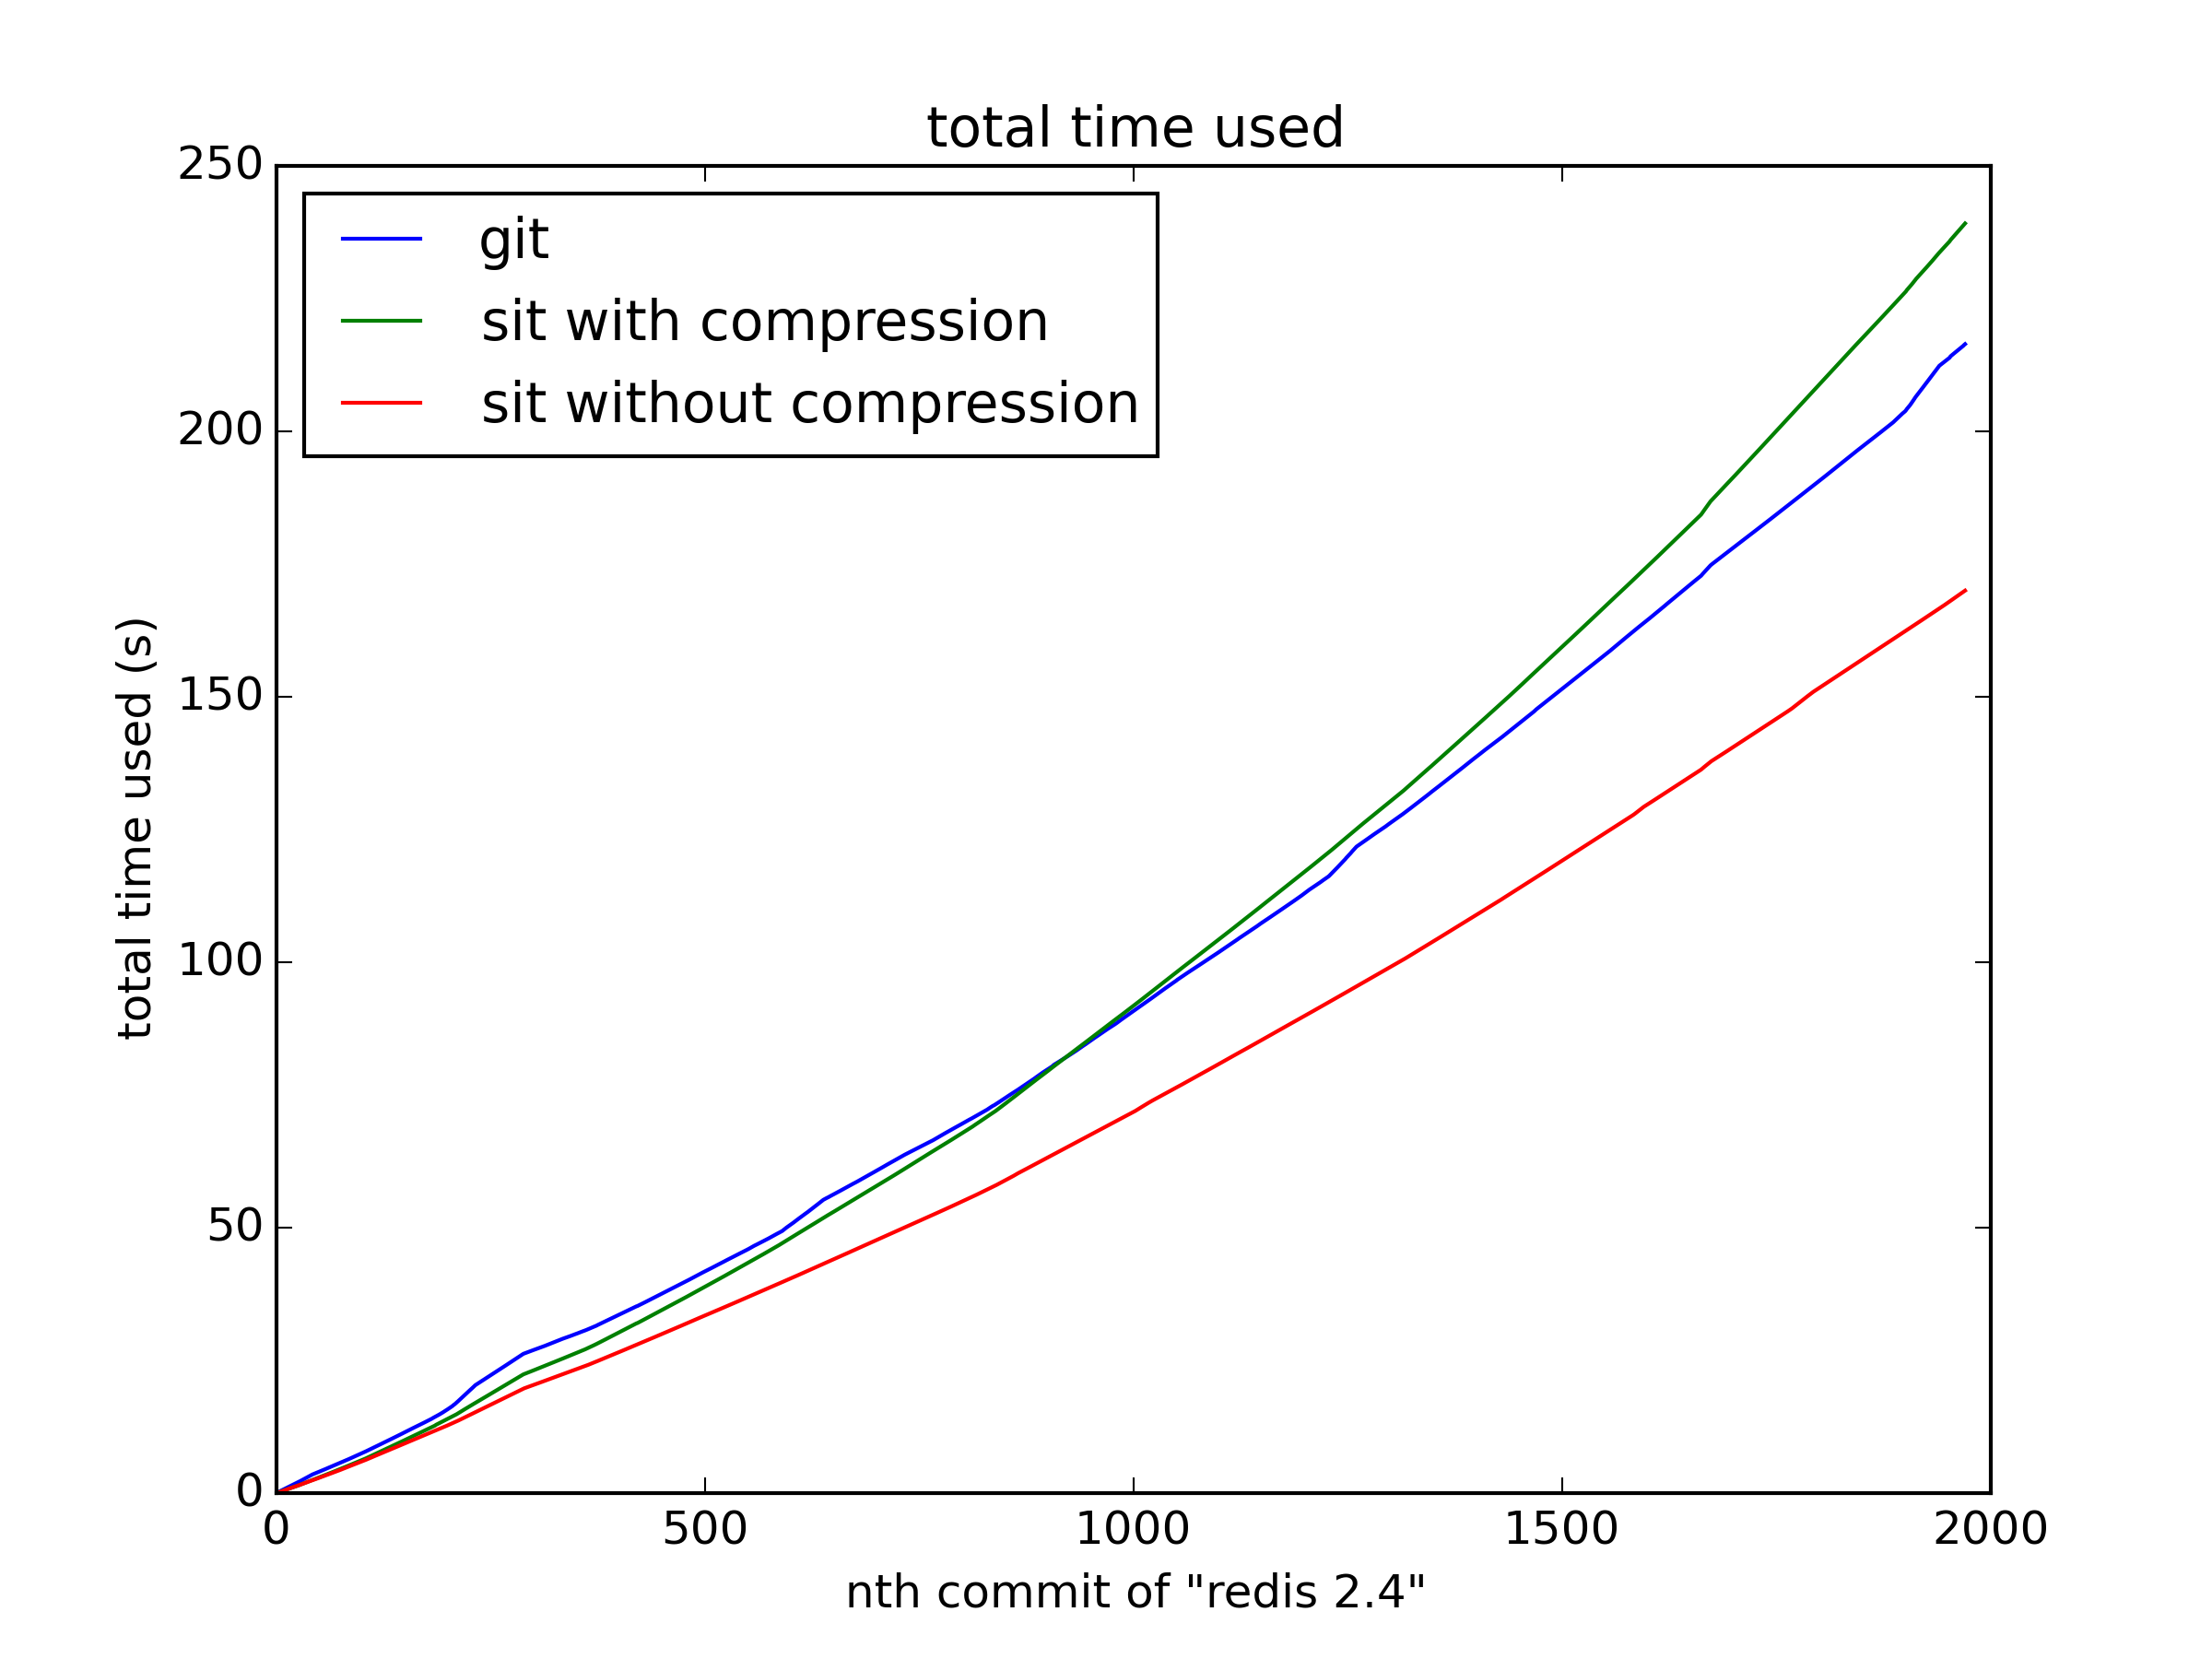
\includegraphics[scale=0.7]{figure_2.png}
	\caption{耗去的总时间}
\end{figure}
\subsection{结论}
从时间和空间的测试结果可以初步得出结论:在不支持压缩时,sit快于git,但仓库占用的空间约为git的2.8倍;支持压缩的sit的运行速度明显下降,低于git,但是在空间效率上升,优git更好。

\section{总结}
在这个编写这个项目的过程中,遇到了不少的困难。考虑到用户的使用体验,我们在设计参数和处理命令的时候增加了很多人性化的设计。就目前来说sit中大量使用了C++STL中的模版来存储各类信息,同时为了保证多平台的支持,使用了boost库来实现与文件系统的交互,因此,在效率上还有一定的提升空间。当然,目前sit的功能还比较孱弱,有一些不人性化的处理还有待完善。
\end{document}